\section{Data Set}
\subsection{Description}
In this study, the data set consists of a set of graphic works for which attribution is established and unambiguous and for which a uniform resolution expressed in \gls{dpi} is known. It was decided to use calligraphic works, as evidenced in \cite{thesis}. The use of calligraphic works represents a promising first way for artistic attribution.

\noindent The dataset used in the reference article consisted of authentic and unaltered handwriting samples. In this study, the dataset consists of university notes, which do not have a sufficiently high standard and therefore present some significant challenges:

\begin{itemize}
\item \textbf{The squares}: Note sheets often contain small squares that could be mistaken for the author's handwriting. This visual interference can complicate the attribution process.
\item \textbf{Use a variety of writing tools}: University notes can be written using a variety of writing tools, such as highlighters, markers, pencils or white-out. These different writing tools produce different lines and colours, which can affect the attribution of authorship.
\item \textbf{Different graphical contexts}: Notes can contain a variety of elements such as mathematical formulae, graphs and erasures. These features represent heterogeneous graphical contexts that add complexity to the analysis.
\item \textbf{Scanning contamination}: The quality of the page scan can introduce blemishes into the record. These blemishes, such as stains or blurring, can affect the clarity and legibility of the works.
\end{itemize}

\noindent In addition, the use of a pen with a thickness of $0.4\operatorname{\mathrm{mm}}$ on the sheet was considered a reasonable first choice since in \cite{thesis} the stroke had the same thickness. This particular aspect is also important in ensuring a certain uniformity and consistency in the visual attributes of the works under examination, thus facilitating a more accurate attribution of authorship.

\noindent The dataset is organised into $4$ authors, and the included images are as follows:

\begin{itemize}
\item The images are saved in the \gls{png} format.
\item Each image is composed of three colour channels \gls{rgb}, each with a depth of 8 bits.
\item The original sheets were scanned at a resolution of 400 \gls{dpi}.
\item The thickness of the pen used to write on the original sheets is $0.4\operatorname{\mathrm{mm}}$.
\end{itemize}

\noindent The images were then cut to remove large impurities or large white spaces. Finally leaving a total of $420$ images.

\begin{table}[h]
    \centering
    \begin{tabular}{|>{\columncolor{pink}}c|c|c|c|}
        \hline
        \rowcolor{lavender}
        \cellcolor{mint} AuthorID & Num of items & Size & Mean side length \\
		\hline
        $1$ & $270$ & $554\operatorname{\mathrm{MB}}$ & $\num{1.43}\operatorname{\mathrm{Kpx}}$ \\
        \hline
        $2$ & $43$ & $133\operatorname{\mathrm{MB}}$ & $\num{1.8}\operatorname{\mathrm{Kpx}}$ \\
        \hline
        $3$ & $56$ & $227\operatorname{\mathrm{MB}}$ & $\num{2.0}\operatorname{\mathrm{Kpx}}$ \\
        \hline
        $4$ & $51$ & $247\operatorname{\mathrm{MB}}$ & $\num{2.2}\operatorname{\mathrm{Kpx}}$ \\
        \hline
        \hline
        \cellcolor{mint} Total & $420$ & $1.2\operatorname{\mathrm{GB}}$ & $\num{1.7}\operatorname{\mathrm{Kpx}}$ \\
        \hline
    \end{tabular}
    \caption[Summary of dataset]{Each item is a cleaned area of the original images. The size represent the total number of pixels. The last column is the geometric mean of the side length, it's compute as follow: $\sqrt{\frac{\text{Num of pixels}}{\text{Num of items}}}$}
\end{table}

In the dataset creation, full clipboard images were collected and then cut to exclude non-pen strokes, highlights, and erasures. In addition, some cuts are particularly small and in a few cases are slightly overlapping.

\begin{figure}[h]
    \centering
    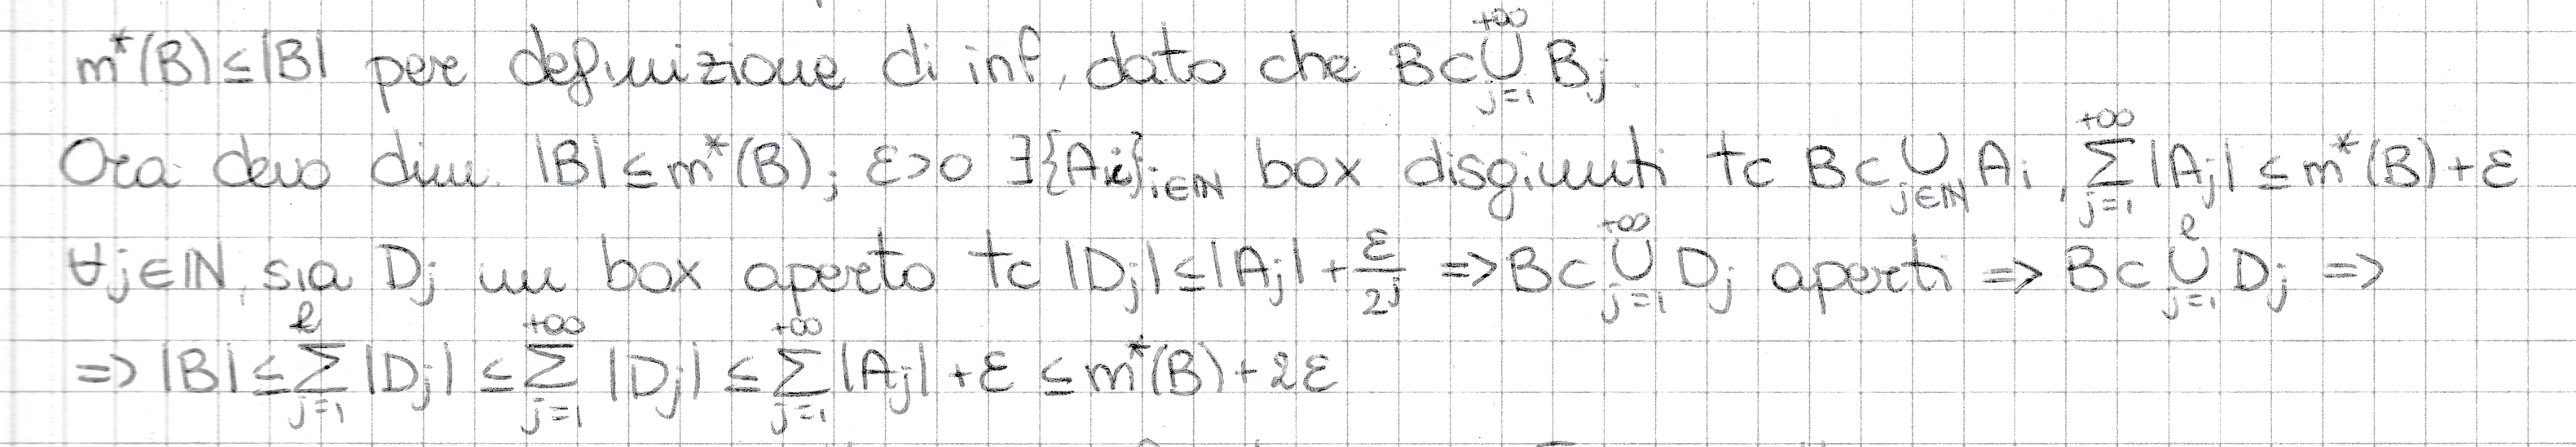
\includegraphics[width=\linewidth]{Figures/Author1_0001_02.png}
\end{figure}
